\section{Algorithms}

This section describes the three algorithms which were benchmarked together with my own algorithm contribution. The Matlab code can be viewed in appendix \ref{appendix:algorithms}.

\subsection{Differential Evolution}

Differential evolution~\cite{Storn1997} is a stochastic optimization algorithm which works on populations of parameter vectors. The problem to minimize will be denoted by $f(x)$ where $X=[x_1,x_2,x_3,...x_D]$ and $D$ is equal to the number of variables taken as input parameters by $f(x)$. The algorithm consists of multiple steps which will be described in detail below.

The first step in DE is to create an initial population, the size of the population is $N$ and it will be represented by a matrix $x$ where $g$ is the generation and $n=1,2,3,...,N$:

\begin{equation}
x_{n,i}^{g} = [ x_{n,1}^{g}, x_{n,2}^{g}, x_{n,3}^{g}, ..., x_{n,D}^{g} ]
\end{equation}

The population is randomly generated to uniformly fill the entire parameter space ($x_{n,i}^U$ is the upper bound for parameter $x_i$ and $x_{n,i}^L$ is the lower bound for parameter $x_i$):

Mutation is the first step when creating a new generation from the population. Mutation is performed individually for every vector $x$ in the population. The mutation procedure is as follows: select three random vectors for each parameter vector (this requires that the population has a size of $N > 3$) and create a set of new vectors $v$ called mutant vectors according to the formula below where $n=1,2,3,...,N$:

\begin{equation}
v_{n}^{g+1} = [ x_{r1n}^{g} + F(x_{r2n}^{g} - x_{r3n}^{g})
\end{equation}

The value of $F$ can be chosen from the interval $[0,2]$ and determines the influence of the differential weight $(x_{r2n}^{g} - x_{r3n}^{g})$.

Crossover occurs after mutation and is applied individually to every vector $x$. A new vector $u$ called the trial vector is constructed from the mutant vector $v$ and the original vector $x$. The trial vector is produced according to the formula below with $i=1,2,3,...,D$ and $n=1,2,3,...,N$:

\begin{equation}
    u_{n,i}^{g+1} =
    \begin{cases}
      v_{n,i}^{g+1}, & \text{if}\ rand() \leq CR \wedge i = I_{\text{rand}} \\
      x_{n,i}^{g}, & \text{otherwise}
\end{cases}
\end{equation}

$I_{\text{rand}}$ is a randomly selected index from the interval $[1,D]$ and $CR$ is the crossover constant which determines the probability that an element is selected from the mutant vector.

Selection is the last step in creating a new generation. The trial vector $u$ is compared with the original vector $x$ for fitness and the vector with the lost cost is selected for the generation according to the formula below where $n=1,2,3,...,N$:

\begin{equation}
    x_{n}^{g+1} =
    \begin{cases}
      u_{n}^{g+1}, & \text{if} f(u_{n}^{g+1}) < f(x_{n}^{g}) \\
      x_{n,i}^{g}, & \text{otherwise}
\end{cases}
\end{equation}

After selection is performed for every vector in the population the population is evaluated to determine if an acceptable solution has been generated. If a solution has been found the algorithm terminates, otherwise the mutation, crossover and selection is performed again until a solution is found or a maximum number of iterations has been reached.

In the benchmark the parameters for DE have been set to $F = 0.6$ and $CR=0.9$ as recommended by Gamperle et al.~\cite{gamperle2002parameter}.

\paragraph{Variants}

Different DE schemes are classified as DE/x/y, where x symbolizes the vector which is mutated and y is the number of differential vectors used. The value of x can be ``rand'' for random vector or ``best''' for the best vector in the population. The algorithm abose is therefore classified as DE/rand/1. The variant DE/best/2 is considered to be a good alternative to DE/rand/1~\cite{qin2009differential}. It's mutation equation is described below:

\begin{equation}
v_{n}^{g+1} = [ x_{best}^{g} + F(x_{r1n}^{g} - x_{r2n}^{g}) + F(x_{r3n}^{g} - x_{r4n}^{g})
\end{equation}

\subsection{Particle Swarm Optimization}

Particle Swarm Optimization (PSO)~\cite{Das2008} was introduced in 1995 by Kenneth and Ebenhart~\cite{eberhart1995new}. The optimization problem is represented by an n-dimensional function

\begin{equation}
  f(x_1,x_2,x_3,...x_n) = f(\vec{X})
\end{equation}

where $\vec{X}$ is a vector which represents the real parameters given to the function. The intent is to find a point in the n-dimensional parameter hyperspace that minimizes the function.

PSO is a parallel search technique where a set of particles  fly through the n-dimensional search space and probe solutions along the way. Each particle $P$ has a current position $\vec{x}(t)$, a current velocity $\vec{v}(t)$, a personal best position $\vec{p}(t)$ and the neighborhoods best position $\vec{g}(t)$. A neighborhood $N$ is a collection of particles which act as independent swarms. Neigborhoods can be social or geographical. Social neigborhoods do not change and contain the same particles during the entire optimization process, while geographical neighborhoods are dynamic and consist only of particles which are near to one another. The neighborhood is often set to be identical to the whole swarm of particles, denoted $S$.

\begin{figure}[H]
  \centering
  \includegraphics[width=.3\linewidth]{pso}
  \caption{Illustration of particles in PSO (red represents the best particle)}
  \label{fig:pso}
\end{figure}

The algorithm has a set of general properties: $v_{max}$ restricts the velocity of each particle to the interval $[-v_{max},v_{max}]$, an inertial factor $\omega$, two random numbers $\phi_1$ and $\phi_2$ which affect the velocity update formula by modulating the influence of $\vec{p}(t)$ and $\vec{g}(t)$, and two constants $C^2$ and $C^1$ which are termed particle “self-confidence” and “swarm confidence”.

The initial values of $\vec{p}(t)$ and $\vec{g}(t)$ are equal to $\vec{x}(0)$ for each particle. After the particle have been initialized an iterative update process is started which modifies the positions and velocities of the particles. The formula below describes the process ($d$ is the dimension of the position and velocity and $i$ is the index of the particle):

\begin{equation}
  v_{id} (t+1) = \omega v_{id} (t) + C_1 \phi_1 (p_{id} (t) - x_{id} (t)) + C_2 \phi_2 (g_{id} (t) - x_{id} (t))
\end{equation}

\begin{equation}
  x_{id} (t+1) = x_{id} (t) + v_{id} (t+1)
\end{equation}

The “self-confidence” constant affects how much self-exploration a particle is allowed to do while “swarm-confidence” affects how much a particle follows the swarm. $\phi_1$ and $\phi_2$ are random numbers which push the particle in a new direction while $\omega$ keeps a particle on the path it’s currently on. The PSO algorithm is described in figure~\ref{algo:pso}. See figure~\ref{fig:pso} for an illustration of PSO.

\begin{figure}[h]
  \centering
  \begin{minipage}{12.5cm}
    \begin{algorithmic}
      \State Init particals with random postitions
      $\vec{x}(0)$ and velocities $\vec{v}(0)$
      \Repeat
        \ForAll{Particles $i$}
          \State Evaluate fitness $f(\vec{x_i})$
          \State Update $\vec{p}(t)$ and $\vec{g}(t)$
          \State Adapt the velocity of the particle using the above-mentioned equation
          \State Update the position of the particle
        \EndFor
      \Until{$\vec{g}(t)$ is a suitable solution}
    \end{algorithmic}
  \end{minipage}
  \caption{PSO algorithm}
  \label{algo:pso}
\end{figure}



In the benchmark the parameters for PSO have been set to $\omega = 0.8$~\cite{shi1998modified}, $c_1 = c_2 = 1.494$~\cite{kennedy1999small} and $v_{max} = \text{parameter range size}$~\cite{Das2008}.

\subsection{Estimation of Distribution Algorithm}

Estimation of distribution algorithms are stochastic search algorithms which try to find the optimal value of a function by creating and sampling probability distributions repeatedly. The first step is creating population $P(0)$ and filling it with solution parameter vectors created from a probability distribution which covers the whole search space uniformly. Then all solutions in $P(g)$ are evaluated and the best solutions $S(g)$ are selected (a threshold variable $t$ is used to determine how many solutions are selected, setting $t=50\%$ means that the best 50\% of the solutions are selected). After selection a probabilistic model $M(g)$ is constructed from $S(g)$ and new solutions $O(g)$ are sampled from $M(g)$. Finally $O(g)$ is incorporated into $P(g)$ The generation counter is incremented $g = g + 1$ and the selection, model and sampling stages are repeated until a suitable solution is found~\cite{Hauschild2011111}.

The most difficult part is constructing the probabilistic model, this will differ for continuous and discreet optimization and a model of appropriate complexity has to be chosen depending on the nature of the problem. The simplest method for continuous EDAs is using a continuous Univariate Marginal Density Algorithm (UMDA). However depending on the complexity of the problem other methods such as Estimation of Baysian Networks (EBNA) can be used~\cite{larranaga2012review}.

\paragraph{UMDA}
The UMDA algorithm is an EDA algorithm which uses a set of independent probability distributions to sample new solution vectors. The probability model can be expressed as a product of the individual probabilities

\begin{equation}
  p(x) = \prod _{d=1}^D {p_d(x_d)}
\end{equation}

where $p(x)$ is the global multivariate density, D is the vector length and $p_d(x_d)$ are the individual univariate marginal densities~\cite{povsik2004estimation}. The algorithm is described in figure~\ref{algo:umda}.

\begin{figure}[h]
  \centering
  \begin{minipage}{12.5cm}
    \begin{algorithmic}
      \State Initialize population P
      \Repeat
        \State Evaluate P
        \State Select the best t\% of P into S
        \State Let m be the mean S
        \State Let s be the standard deviation of S
        \State Sample S' from normal distribution using m and s
        \State Create new generation of P from S' and S
      \Until{Termination condition}
    \end{algorithmic}
  \end{minipage}
  \caption{UMDA algorithm}
  \label{algo:umda}
\end{figure}


\subsection{Improved Algorithm: Differential EDA}

My improved algorithm, differential EDA (DEDA), draws upon DE and EDA, applying differential mutation to the selection population of the EDA algorithm. The algorithm is described in figure~\ref{algo:my}.


\begin{figure}[h]
  \centering
  \begin{minipage}{12.5cm}
    \begin{algorithmic}
      \State Initialize random population $P$
      \Repeat
        \State Sort population $P$
        \State Select $S$ from $P$
        \State Build probabilistic model $M$ from $S$
        \State Sample $P'$ from $M$
        \State Let $S_{DE}$ be DE applied to $S$
        \State Create new generation $P$ from $P'$ and $S_{DE}$
      \Until{Termination condition}
    \end{algorithmic}
  \end{minipage}
  \caption{Improved algorithm}
  \label{algo:my}
\end{figure}



\section{Mathematical Problem Set}

The functions for the benchmark are taken from the 2005 CEC conference on continuous evolutionary optimization~\cite{suganthan2005problem}. The functions are losely based on the popular optimization benchmark suite created by DeJong~\cite{Whitley1996245}.

For all functions $x=[x_1,x_2,x_3,...,x_D]$ are the input parameters, $o=[o_1,o_2,o_3,...,o_D]$ is the global optimum, $D$ is the dimension and $M$ is an orthogonal matrix with parameters unique to each function. The matrices for $o$ and $M$ can be obtained from~\cite{suganthan2005problem}. Illustrations of the functions can be found in figures~\ref{f1},~\ref{f2},~\ref{f3},~\ref{f4},~\ref{f5},~\ref{f6},~\ref{f7},~\ref{f8},~\ref{f9} and~\ref{f10}.

The function properties are described in figure~\ref{math:prop}.

\begin{figure}[H]
  \centering
  \begin{center}
    \begin{tabular}{ | c | c | c | }
      \hline
      Function & Modal & Separable \\ \hline
      $F_{1}$ & Uni & Yes \\ \hline
      $F_{2}$ & Uni & No \\ \hline
      $F_{3}$ & Uni & No \\ \hline
      $F_{4}$ & Uni & No \\ \hline
      $F_{5}$ & Uni & No \\ \hline
      $F_{6}$ & Multi & No \\ \hline
      $F_{7}$ & Multi & No \\ \hline
      $F_{8}$ & Multi & No \\ \hline
      $F_{9}$ & Multi & Yes \\ \hline
      $F_{10}$ & Multi & No \\

      \hline
    \end{tabular}
  \end{center}
  \caption{Function properties}
  \label{math:prop}
\end{figure}

\subsection{$F_1$: Shifted Sphere Function}

\begin{equation}
  F_1(x)=\sum_{i=1}^{D}{z_i^2}
\end{equation}
\[ z=x-o \]
\[ x \in [-100,100]^D \]

\begin{figure}[H]
  \centering
  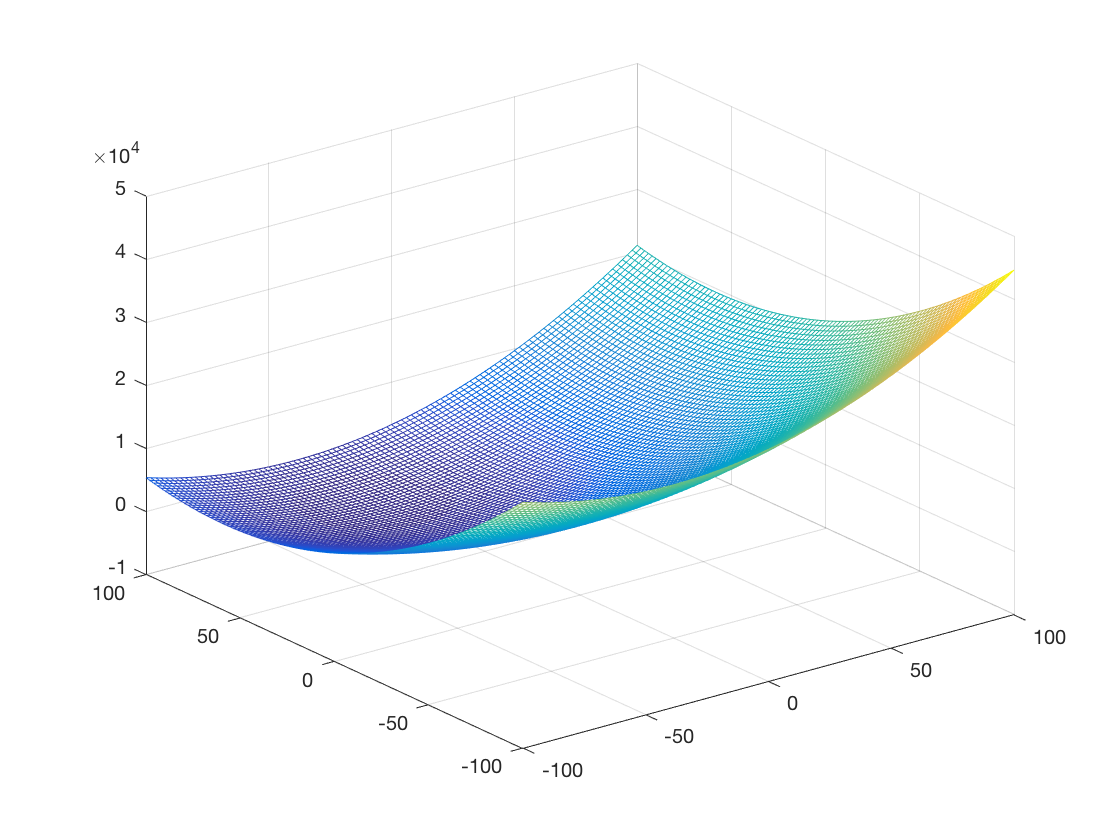
\includegraphics[width=.3\linewidth]{f1}
  \caption{3-D map for 2-D function}
  \label{f1}
\end{figure}

\subsection{$F_2$: Shifted Schwefel’s Problem}

\begin{equation}
  F_2(x)=\sum_{i=1}^{D}{(\sum_{j=1}^{i}{z_j})^2}
\end{equation}
\[ z=x-o \]
\[ x \in [-100,100]^D \]

\begin{figure}[H]
  \centering
  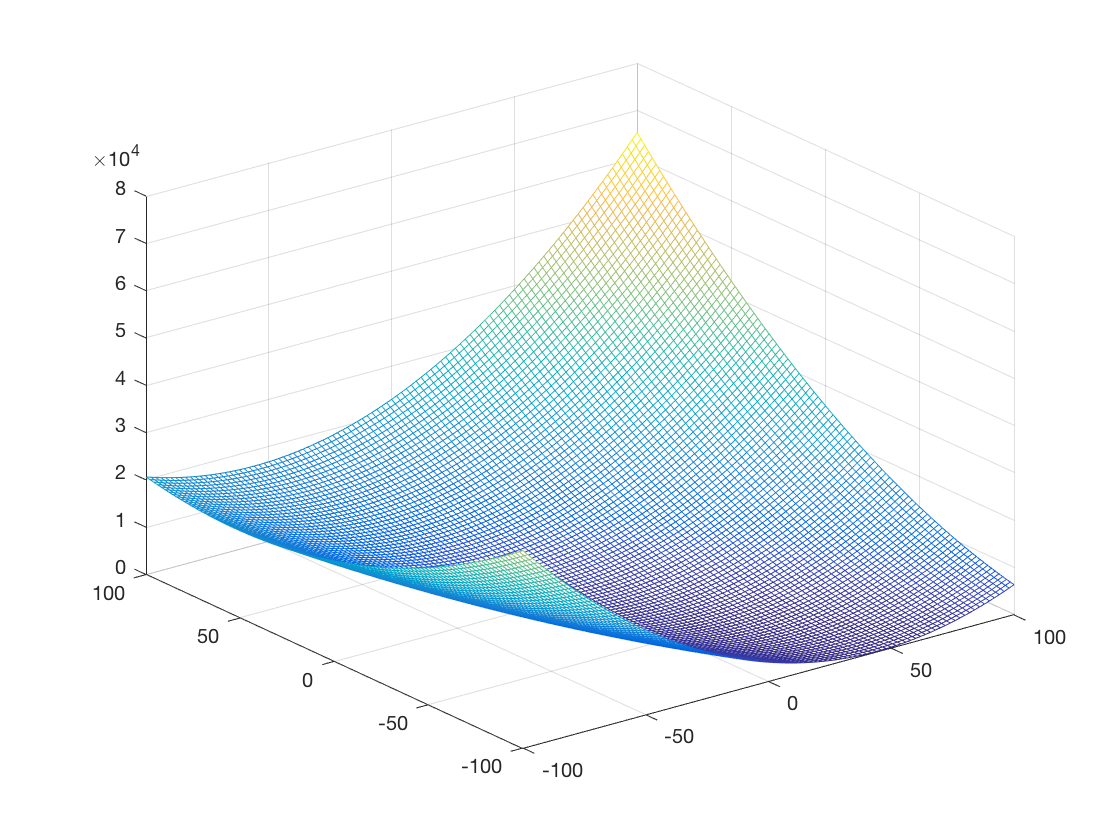
\includegraphics[width=.3\linewidth]{f2}
  \caption{3-D map for 2-D function}
  \label{f2}
\end{figure}

\subsection{$F_3$: Shifted Rotated High Conditioned Elliptic Function}

\begin{equation}
  F_3(x)=\sum_{i=1}^{D}{(10^6)^{\frac{i-1}{D-1}}z_i^2}
\end{equation}
\[ z=(x-o)*M \]
\[ x \in [-100,100]^D \]

\begin{figure}[H]
  \centering
  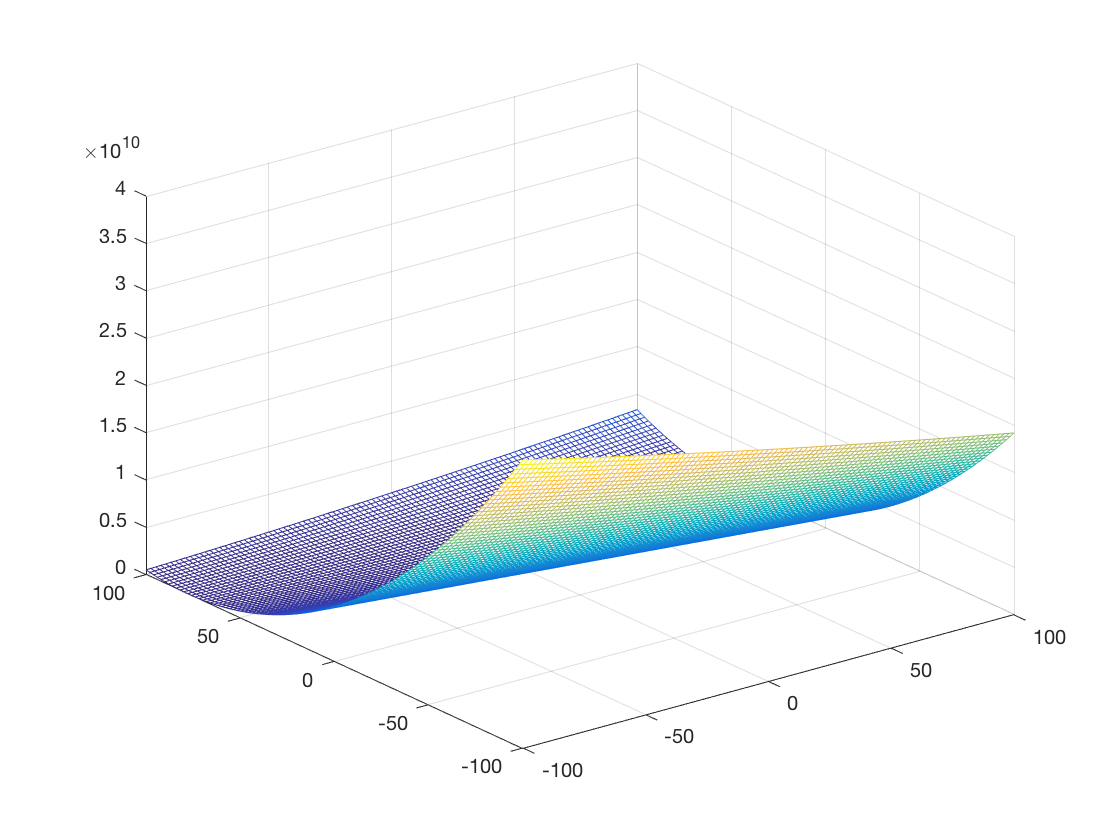
\includegraphics[width=.3\linewidth]{f3}
  \caption{3-D map for 2-D function}
  \label{f3}
\end{figure}

\subsection{$F_4$: Shifted Schwefel’s Problem with Noise in Fitness}

\begin{equation}
  F_4(x)=(\sum_{i=1}^{D}{(\sum_{j=1}^{i}{z_j})^2})*(1+0.4|N(0,1)|)
\end{equation}
\[ z=x-o \]
\[ x \in [-100,100]^D \]

\begin{figure}[H]
  \centering
  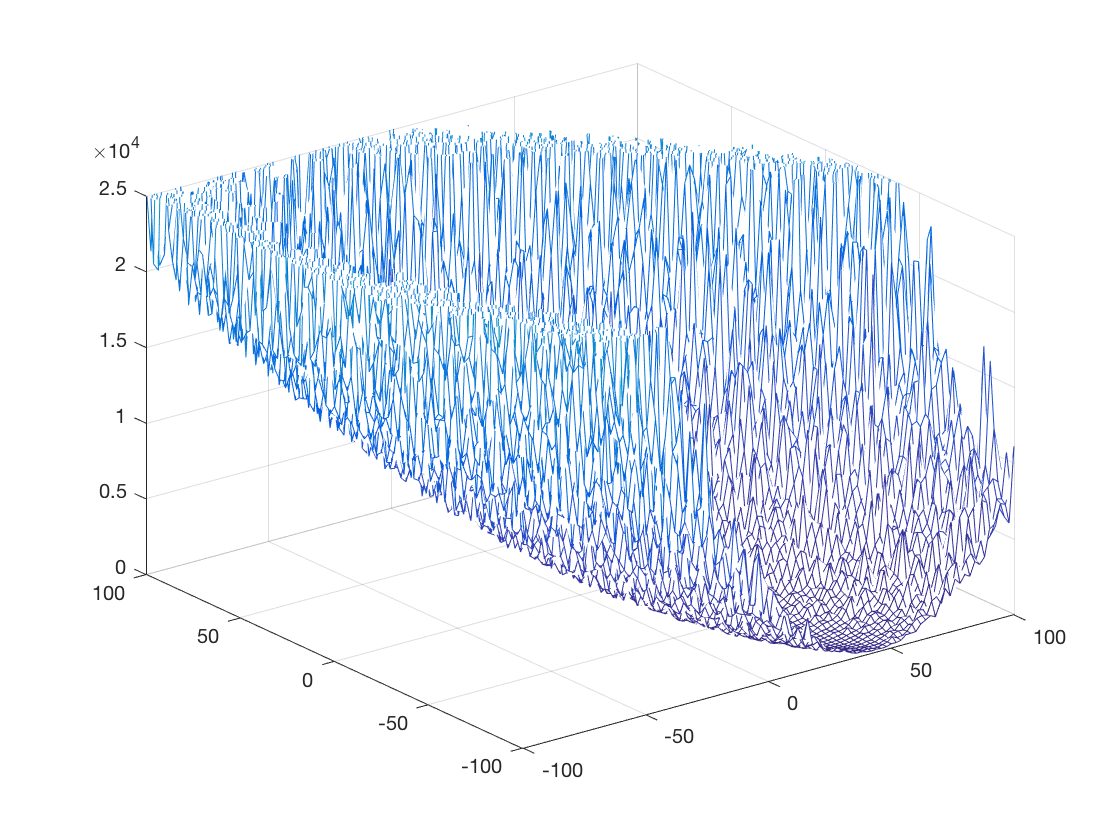
\includegraphics[width=.3\linewidth]{f4}
  \caption{3-D map for 2-D function}
  \label{f4}
\end{figure}

\subsection{$F_5$: Schwefel’s Problem with Global Optimum on Bounds}

\begin{equation}
  F_5(x)=max\{|A_ix-B_i|\}
\end{equation}
\[ i=1,...,D, x \in [-100,100]^D \]
\[ A \text{ is a } D*D \text{ matrix}, a_{ij} = \text{ random numbers in } [-500,500],  det(A) \neq 0 \]
\[ B_i = A_i * o, o_i = \text{ random numbers in } [-100,100] \]
\[ o_i = -100 \text{, for } i=1,2,...,[D/4], o_i = 100 \text{, for } i=[3D/4],...,D \]

\begin{figure}[H]
  \centering
  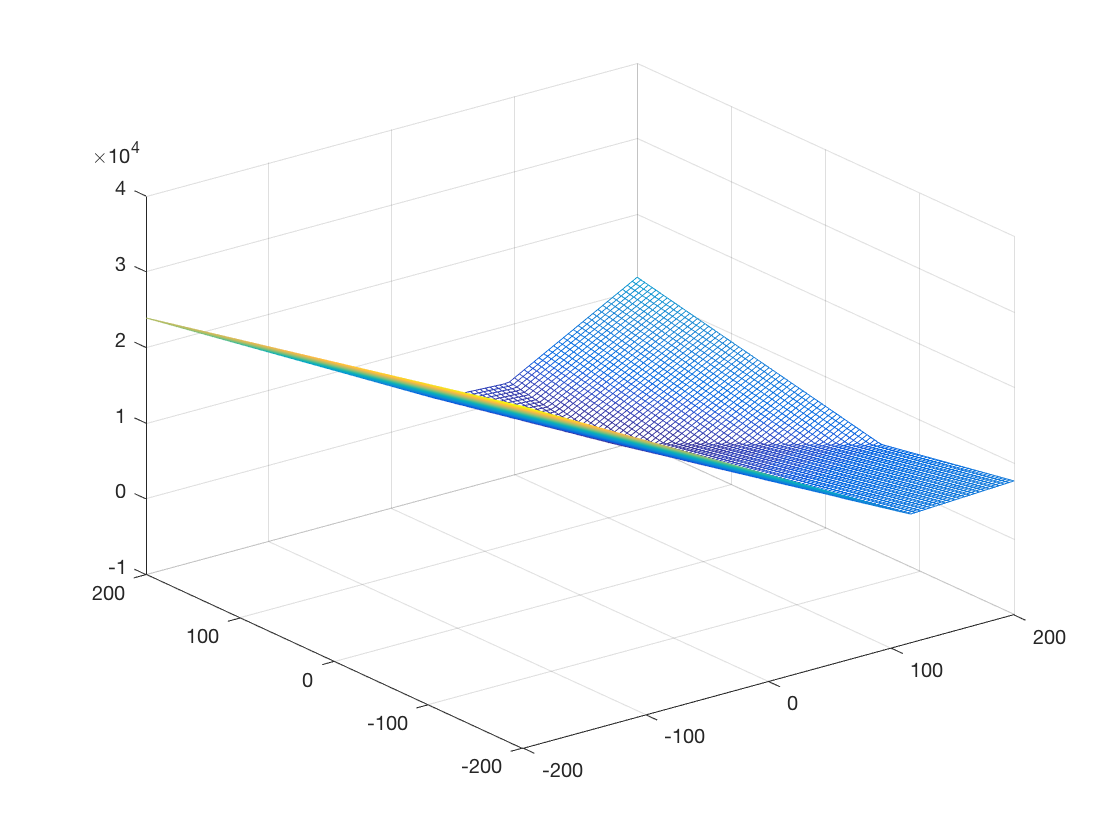
\includegraphics[width=.3\linewidth]{f5}
  \caption{3-D map for 2-D function}
  \label{f5}
\end{figure}

\subsection{$F_6$: Shifted Rosenbrock’s Function}

\begin{equation}
  F_6(x)=\sum_{i=1}^{D-1}{(100(z_i^2 - z_{i+1})^2 + (z_i - 1)^2)}
\end{equation}
\[ z=x-o+1 \]
\[ x \in [-100,100]^D \]

\begin{figure}[H]
  \centering
  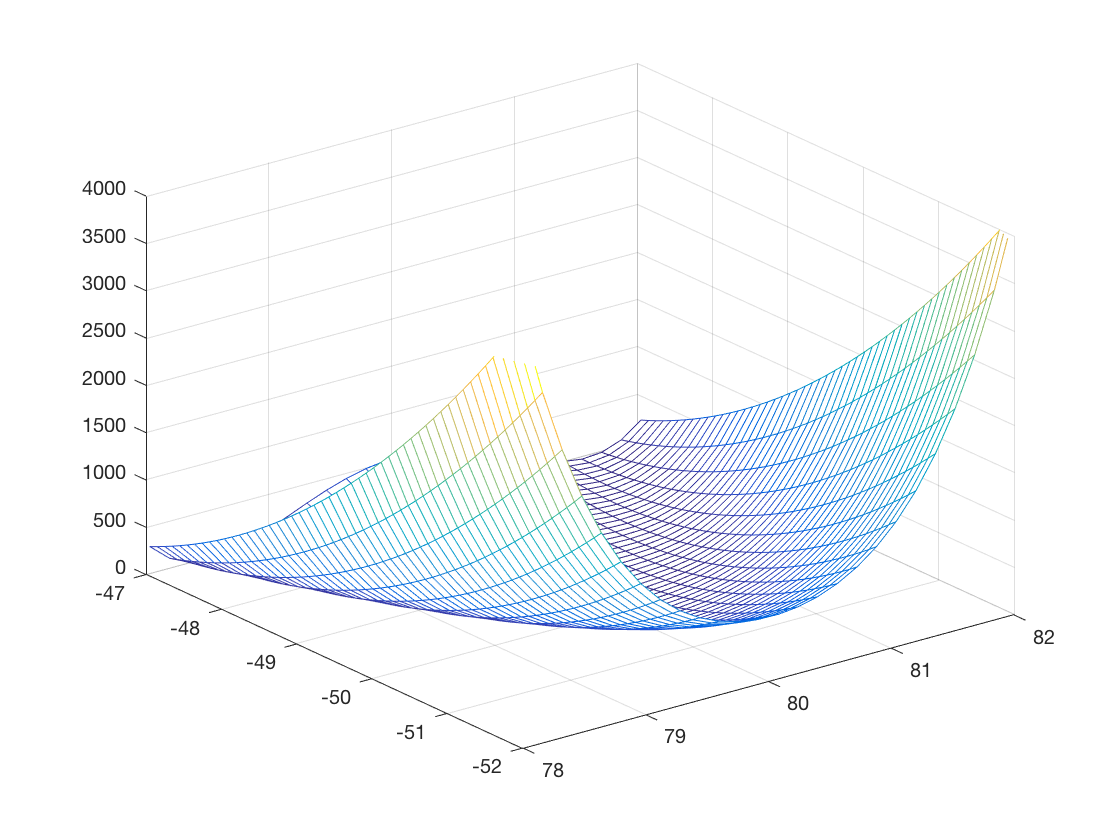
\includegraphics[width=.3\linewidth]{f6}
  \caption{3-D map for 2-D function}
  \label{f6}
\end{figure}

\subsection{$F_7$: Shifted Rotated Griewank’s Function without Bounds}

\begin{equation}
  F_7(x)=\sum_{i=1}^{D}{\frac{z_i^2}{4000}}-\prod_{i=1}^{D}{\cos{\frac{z_i}{\sqrt{i}}}}+1
\end{equation}
\[ z=(x-o)*M \]
\[ x \in [0,600]^D \]

\begin{figure}[H]
  \centering
  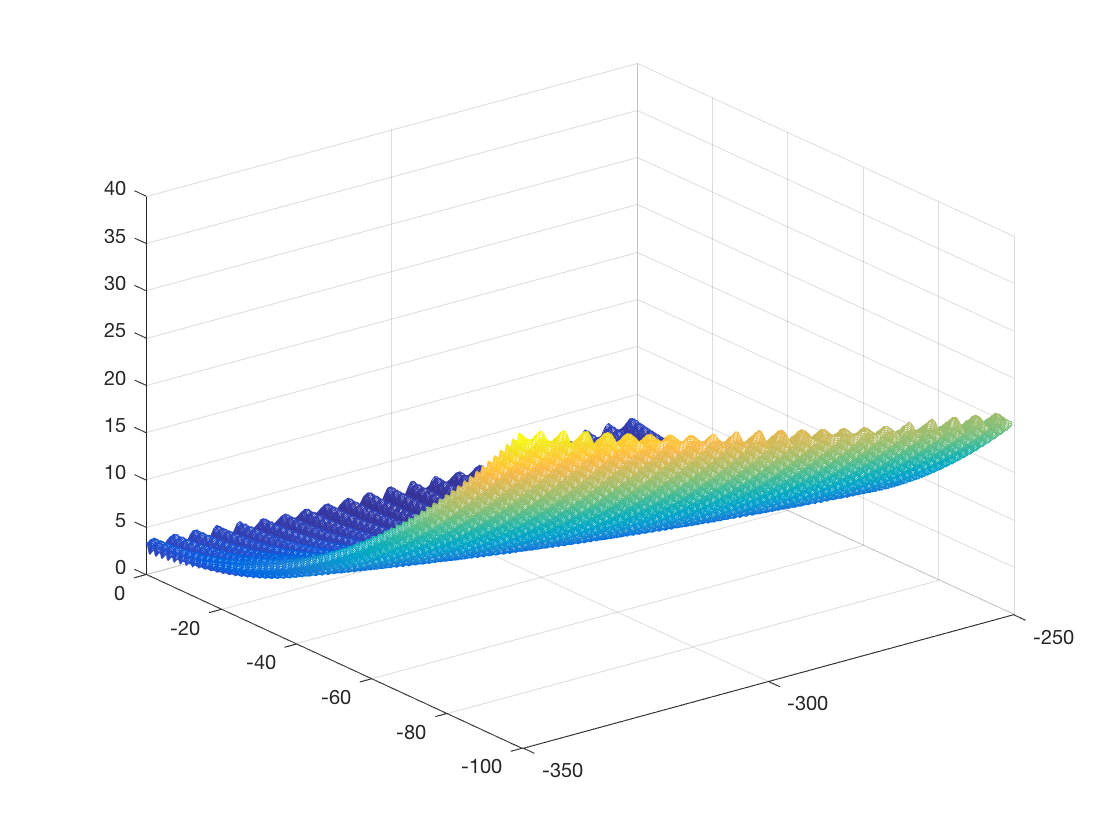
\includegraphics[width=.3\linewidth]{f7}
  \caption{3-D map for 2-D function}
  \label{f7}
\end{figure}

\subsection{$F_8$: Shifted Rotated Ackley’s Function with Global Optimum on Bounds}

\begin{equation}
  F_8(x)=-20\exp{(-0.2\sqrt{\frac{1}{D}\sum_{i=1}^{D}{z_i^2}})}-\exp{(\frac{1}{D}\sum_{i=1}^{D}{\cos{(2\pi z_i)}})} + 20 + e
\end{equation}
\[ z=(x-o)*M \]
\[ x \in [-32,32]^D \]

\begin{figure}[H]
  \centering
  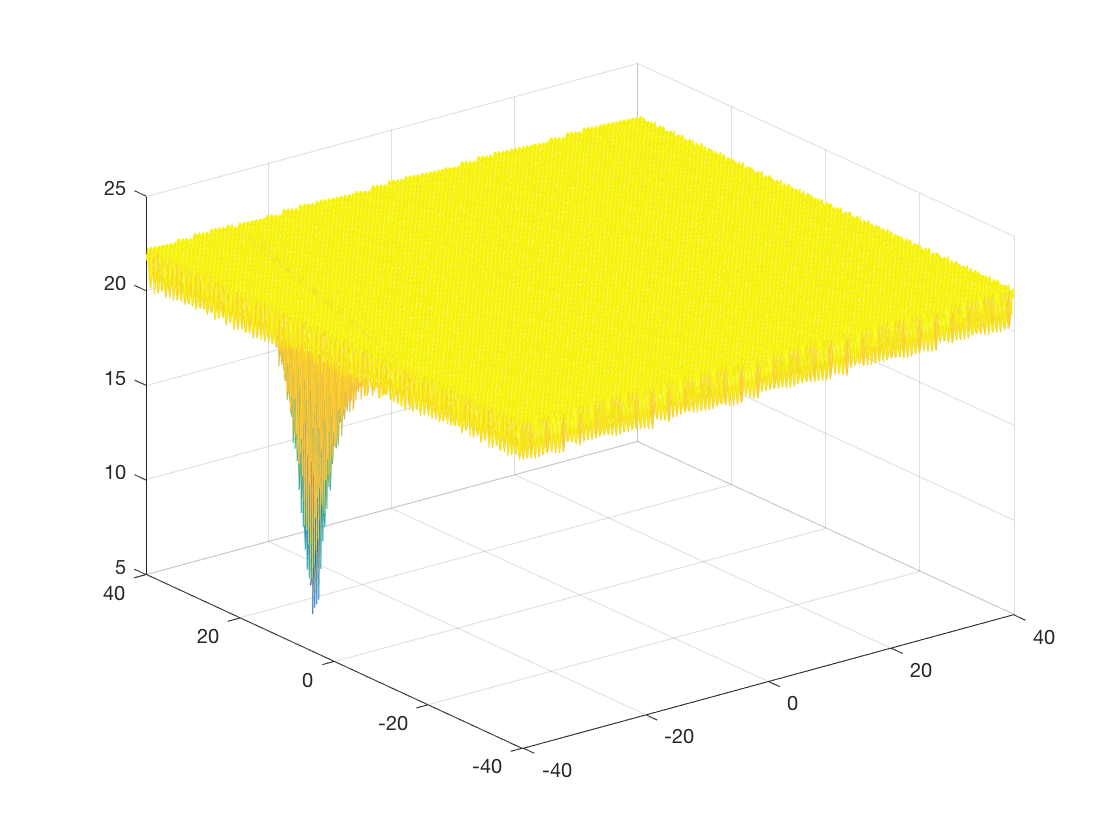
\includegraphics[width=.3\linewidth]{f8}
  \caption{3-D map for 2-D function}
  \label{f8}
\end{figure}

\subsection{$F_9$: Shifted Rastrigin’s Function}

\begin{equation}
  F_9(x)=\sum_{i=1}^{D}{z_i^2 - 10\cos{(2\pi z_i)} + 10}
\end{equation}
\[ z=x-o \]
\[ x \in [-5,5]^D \]

\begin{figure}[H]
  \centering
  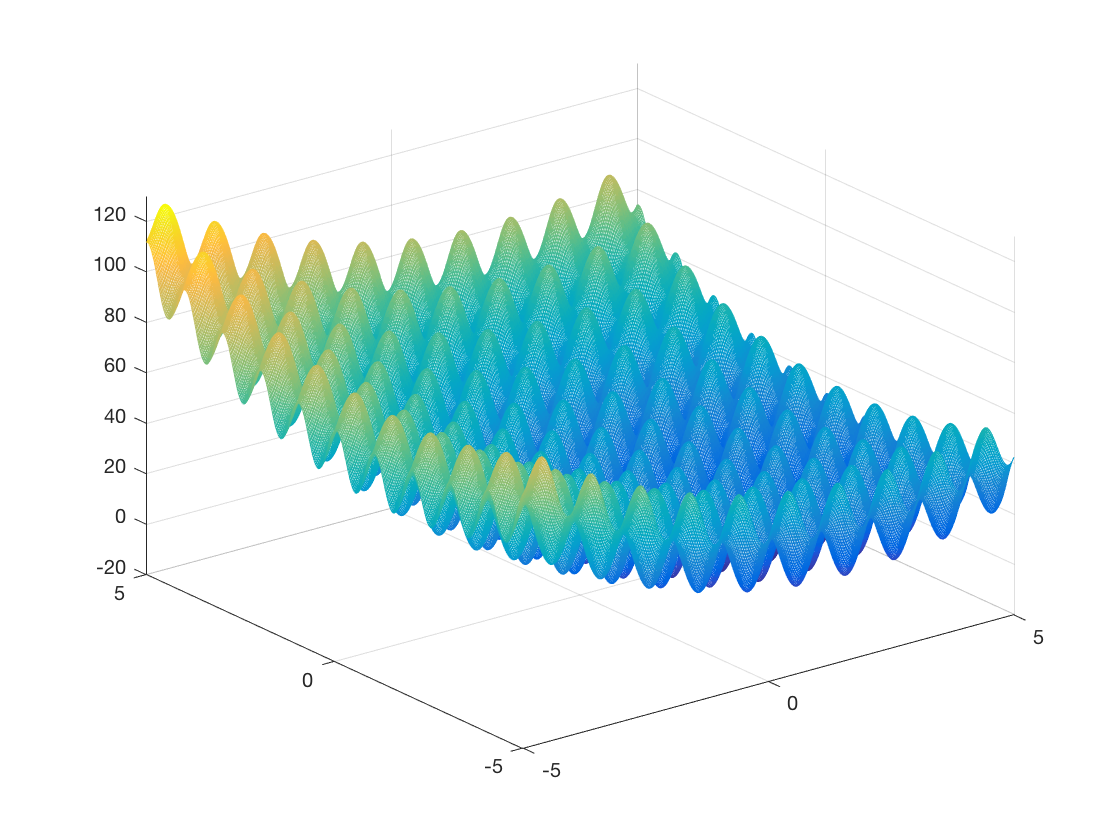
\includegraphics[width=.3\linewidth]{f9}
  \caption{3-D map for 2-D function}
  \label{f9}
\end{figure}

\subsection{$F_{10}$: Shifted Rotated Rastrigin’s Function}

\begin{equation}
  F_{10}(x)=\sum_{i=1}^{D}{z_i^2 - 10\cos{(2\pi z_i)} + 10}
\end{equation}
\[ z=(x-o)*M \]
\[ x \in [-5,5]^D \]

\begin{figure}[H]
  \centering
  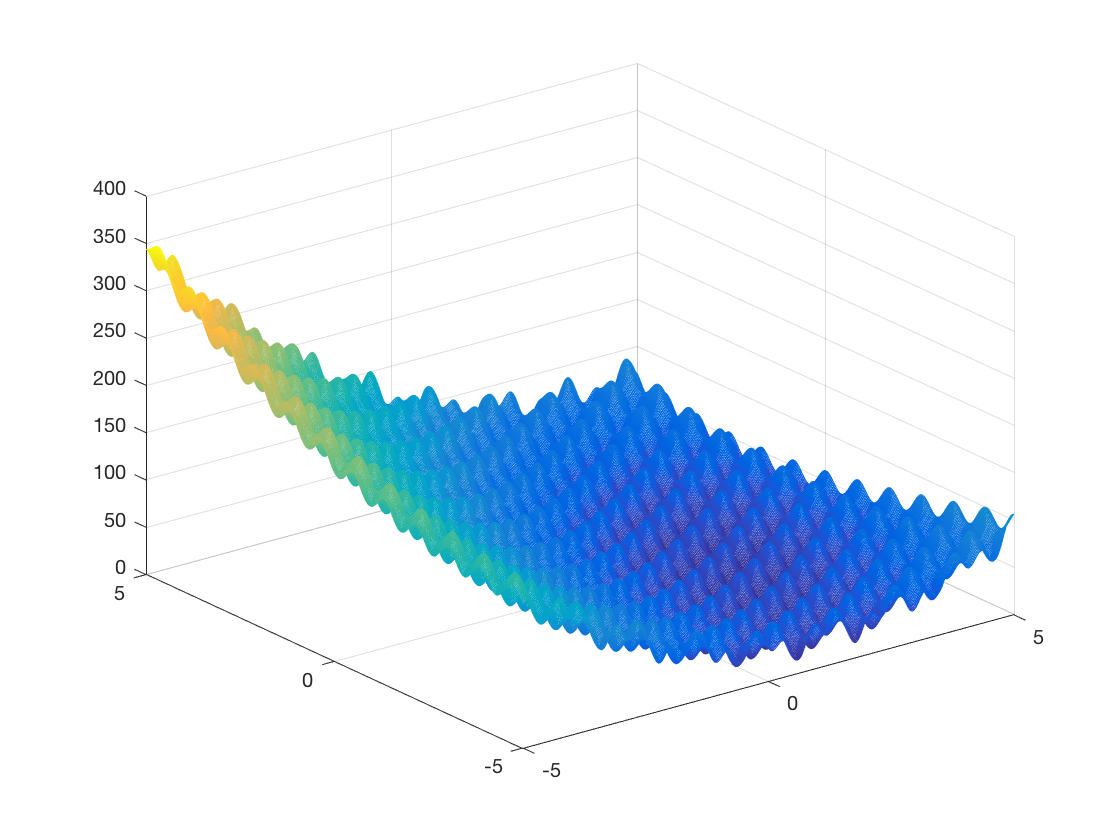
\includegraphics[width=.3\linewidth]{f10}
  \caption{3-D map for 2-D function}
  \label{f10}
\end{figure}

\section{Machine Learning Problem Set}

To evaluate the optimization algorithms further I set have set out to apply them on a variety of machine learning problems. These will predominantly be applications of feed-forward neural networks (FFNN). The design of the neural network is one input layer with a size based on the problem dimension, two hidden layers and one output layer. I have chosen to use two hidden layers to make sure a good solution can be found quickly~\cite{329294}. The size of the hidden layers was set to $2/3$ and $1/3$ of the mean of the size of the input and output layers.

\subsection{$ML_{1}$: Training FFNNs to do function approximation}

The optimization algorithm were used to train FFNNs to perform function approximation and curve-fitting on seven sample data-sets which are available in Matlab's Neural Network Toolbox. The data-sets used are the following

\begin{enumerate}
  \item simplefit\_dataset (Simple fitting dataset)
  \item abalone\_dataset (Abalone shell rings dataset)
  \item bodyfat\_dataset (Body fat percentage dataset)
  \item building\_dataset (Building energy dataset)
  \item chemical\_dataset (Chemical sensor dataset)
  \item cho\_dataset (Cholesterol dataset)
  \item engine\_dataset (Engine behavior dataset)
  \item house\_dataset (House value dataset)
\end{enumerate}

The data sets contain two matrices. One with sample input vectors to the neural network and one with the expected correct output vectors. The function which the optimization algorithm directly optimize is the sum of squared errors as defined by

\begin{equation}
  sse(x,t) = \frac{1}{2n} \sum_{i=1}^{n}{(y(x)-t)^2}
\end{equation}

where $x$ is the input vector to neural network $y$, $t$ is the correct expected output which $y(x)$ should produce and n is the length of vector $x$.

\subsection{$ML_{2}$: Training FFNNs to do classification}

The optimization algorithm were used to train FFNNs to perform classification tasks on eight sample data-sets which are available in Matlab's Neural Network Toolbox. The data-sets used are the following

\begin{enumerate}
  \item simpleclass\_dataset(Simple pattern recognition dataset)
  \item cancer\_dataset (Breast cancer dataset)
  \item crab\_dataset (Crab gender dataset)
  \item glass\_dataset (Glass chemical dataset)
  \item iris\_dataset (Iris flower dataset)
  \item thyroid\_dataset (Thyroid function dataset)
  \item wine\_dataset (Italian wines dataset)
\end{enumerate}

The evaluation procedure is the same as for $ML_{1}$.

\subsection{$ML_{3}$: Training FFNNs to do clustering}

The optimization algorithm were used to train FFNNs to perform clustering tasks on one sample data-sets which is available in Matlab's Neural Network Toolbox. The data-sets used is the following

\begin{enumerate}
  \item simplecluster\_dataset (Simple clustering dataset)
\end{enumerate}

The evaluation procedure is the same as for $ML_{1}$ and $ML_{2}$.


\subsection{$ML_{4}$: Neuroevolution of Game Controller for ``Snake''}

Machine learning test set $ML_{1}$ uses evolutionary algorithms to evolve weights for feed-forward neural networks, which control the behavior of game-agent in the classic game of ``Snake''.

\subsubsection{Game Description and Rules}

The game is made up of a $n*m$ square grid through which a snake can freely move. The snake consists of a sequence of interconneted blocks and is divided into a head which moves in a certain direction and a tail which follows the head. Food blocks randomly appear on block at a time on the grid and the snake's objective is eat these blocks. When the snake's head touches the food block the block vanishes and the snake grows one square in length. If the head of the snake tries to move outside the grid it dies and the game ends. If the head of the snake collides with the tail it also and dies and the game ends. The snake's head can move in four direction: up, down, left and right. If the snake tries to move in the opposite of it's currect direction it also dies. The snake has a starvation counter which forces it to pursue food and eat. The starvation counter is initialized to the starvation threshold when the game begins and decreases by one every time the snake moves. When the snake eats, the starvation counter is increased once by the starvation threshold. Figure~\ref{snake} illustrates the game grid. Figure~\ref{snake_alg} described the algorithm for the game.

\begin{figure}[H]
  \centering
  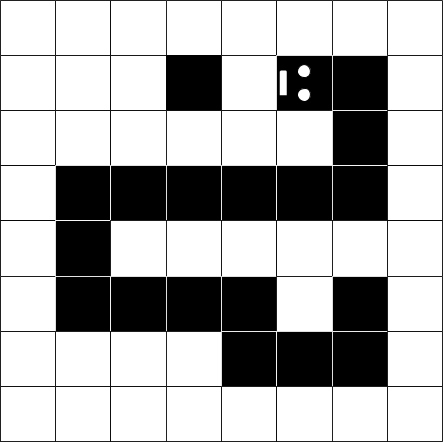
\includegraphics[width=.3\linewidth]{snake}
  \caption{Snake $8*8$ game-field with snake hunting food}
  \label{snake}
\end{figure}

The game has the following parameters and settings:

\begin{enumerate}
  \item Dimensions - $n*m$ blocks in the grid
  \item Starting point $(x,y)$ for snake head
  \item Starting direction for snake head $\{left,right,up,down\}$
  \item Starvation threshold $t$
\end{enumerate}

\subsubsection{Representation of Game State}

In order to control the snake with a neural network a representation of the state of the game has to be generated before each move. The chosen representation is a 12-dimensinal vector in the range $[0,1]$. The initial default value of all dimensions is zero. Dimensions 1-4 indicates with a value of one whether any dangerous object (the tail or the edge of the grid) is immediatly to the left, to the right, above or below the snake's head. Dimensions 5-8 indicate the distribution of the tail relative to the head of the snake. Floating-point numbers indicate how much of the tail is above, below, to the right and to the left of the head. Dimensions 9-12 indicate with a value of one when food is to the left, to the right, above or below the snake's head.

\begin{figure}[h]
  \centering
  \begin{minipage}{12.5cm}
    \begin{algorithmic}
      \State $initializeSnake()$
      \State $foodEaten \gets 0$
      \State $movesMade \gets 0$
      \While{$alive$}
        \State $state \gets getGameState()$
        \State $move \gets getNextMove(state)$
        \State $moveSnake(move)$
        \If{$collides(head,tail)$} $die()$
        \EndIf
        \If{$outOfBounds(head)$} $die$
        \EndIf
        \If{$collides(head,food)$}
          \State{$eatFood(food)$}
          \State{$growSnake()$}
          \State{$foodEaten \gets foodEaten + 1$}
        \EndIf
        \State{$movesMade \gets movesMade + 1$}
      \EndWhile
      \State{\Return $foodEaten + sigmoid(movesMade)$}

    \end{algorithmic}
  \end{minipage}
  \caption{Snake game}
  \label{snake_alg}
\end{figure}

\subsubsection{Neural Network Controller}

The neural network which controls is a feed-forward neural network with one hidden layer. The input layer has 12 neurons which correspond to the game-state representation. The output layer has four neurons, which correspond to the decision to move left, right, up or down. The hidden layer has 8 neurons. Figure \ref{ffnn_snake} illustrates the network.





\begin{figure}[H]
  \centering

  \begin{tikzpicture}[shorten >=1pt,->,draw=black!50, node distance=\layersep]
      \tikzstyle{every pin edge}=[<-,shorten <=1pt]
      \tikzstyle{neuron}=[circle,fill=black,minimum size=14pt,inner sep=0pt]
      \tikzstyle{input neuron}=[neuron];
      \tikzstyle{output neuron}=[neuron];
      \tikzstyle{hidden neuron}=[neuron];
      \tikzstyle{annot} = [text width=2em, text centered]

      % Draw the input layer nodes
      \foreach \name / \y in {1,...,12}
      % This is the same as writing \foreach \name / \y in {1/1,2/2,3/3,4/4}
          \node[input neuron, pin=left:Input \#\y] (I-\name) at (0,-\y) {};

      % Draw the hidden layer nodes
      \foreach \name / \y in {1,...,8}
          \path[yshift=-2cm]
              node[hidden neuron] (H-\name) at (4\layersep,-\y cm) {};

      % Draw the hidden layer nodes
      \foreach \name / \y in {1,...,4}
          \path[yshift=-4cm]
              node[output neuron, pin={[pin edge={->}]right:Output}, right of=H-3] (O-\name) at (8\layersep,-\y cm) {};


      % Connect every node in the input layer with every node in the
      % hidden layer.
      \foreach \source in {1,...,12}
          \foreach \dest in {1,...,8}
              \path (I-\source) edge (H-\dest);

      % Connect every node in the hidden layer with the output layer
      \foreach \source in {1,...,8}
          \foreach \dest in {1,...,4}
              \path (H-\source) edge (O-\dest);
  \end{tikzpicture}

  \caption{FFNN snake controller}
  \label{ffnn_snake}
\end{figure}

\subsubsection{Fitness Function and Evaluation}

The objective function, which is run by the optimization algorithms, takes the evolved weights of the neural network and attempts to play the game using them. The fitness function of gameplay if determined by the equation below:

\begin{equation}
  fitness = \text{foodEaten} + \frac{1}{1-e^{-\text{movesMade}}}
\end{equation}

The fitness function ensured that the snake has an ``easy start'' when it will be revarded for not dying, but then has to pursue food in order to maximize it's fitness.
